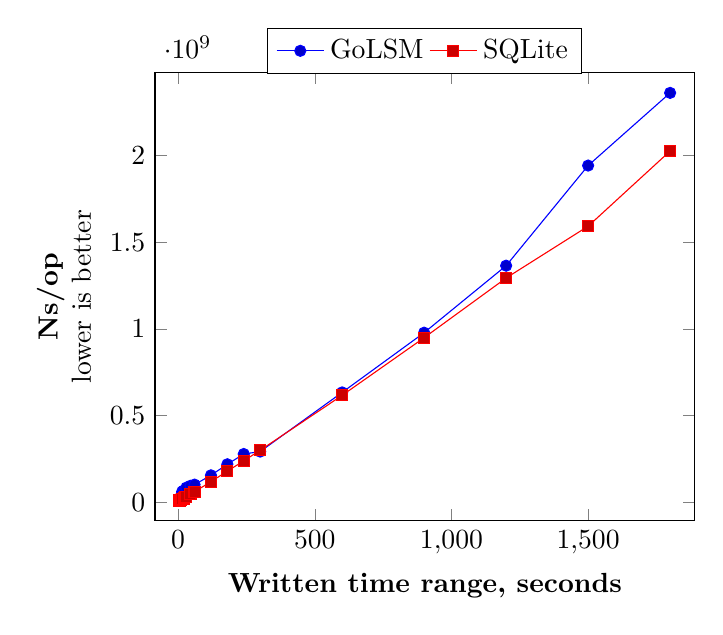
\begin{tikzpicture}
        % first provide your data as table, so later the data can
        % easily be accessed for various stuff
        \pgfplotstableread{
            x    y  z
5 20066750			    9514015
10 34790230			    10956443
15 61277403			    19290607
20 66074549			    20865090
25 63925416			    28999975
30 83572878			    30478476
45 94080339			    48656675
60 100926498			    59882936
120 154617448			    117794298
180 218391345			    178663220
240 277609792			    238031796
300 291599762			    299054072
600 633156270			    616109936
900 977887157			    948873690
1200 1364639379			    1293479495
1500 1942545058			    1592474416
1800 2362087783			    2026594877


        }{\data}
    \begin{axis}[
        x tick style={/pgf/number format/1000 sep=},
	    ylabel style={align=center},	
	    ylabel = \textbf{Ns/op}\\lower is better,
	    xlabel style={align=center},	
	    xlabel = \textbf{Written time range, seconds},
	    enlargelimits=0.05,
	    legend style={
	        at={(0.5,1.1)}, anchor=north,legend columns=-1
	    },
    ]
        % then your `\addplot commands change to
        \addplot table [x=x,y=y] {\data};
        \addlegendentry{GoLSM}
        \addplot table [x=x,y=z] {\data};
        \addlegendentry{SQLite}
    \end{axis}
\end{tikzpicture}